\documentclass[11pt, a4paper]{article}
\usepackage[T2A]{fontenc}
\usepackage[utf8]{inputenc}
\usepackage[bulgarian, english]{babel}

%% Sets page size and margins
\usepackage[a4paper,top=3cm,bottom=3cm,left=3cm,right=3cm,marginparwidth=1.75cm]{geometry}

%% Useful packages
\usepackage{amsmath, amssymb, amsthm,calc,mathabx}
\usepackage{systeme}
\usepackage{graphicx}
\usepackage[colorinlistoftodos]{todonotes}
\usepackage[colorlinks=true, allcolors=black]{hyperref}
\usepackage{wrapfig,lipsum,booktabs}
\usepackage{enumitem}
\usepackage{float}
\usepackage{fmtcount}
\usepackage{multicol}
\usepackage{breqn}
\usepackage{setspace}
\usepackage{hyperref}
\usepackage {tikz}
	\usetikzlibrary {positioning}
	
\graphicspath{
	{Graphics/}
}

\newtheorem{theorem}{Theorem}

\newtheorem{lemma}{Lemma}
\newtheorem{prop}{Property}
\newtheorem*{remark}{Remark}

\theoremstyle{definition}
\newtheorem{definition}{Definition}

\setlength{\columnsep}{1cm}
\setlength{\parindent}{1em}

\begin{document}
\begin{titlepage}
	\newcommand{\HRule}{\rule{\linewidth}{0.5mm}}
	\centering
	\textsc{\LARGE SRS 2019}\\[1cm]
	\HRule\\[1 cm]
	
	{\huge\bfseries Ransomware Research Project }\\[0.5 cm] 
	\HRule\\
    \vfill
			\Large
			\textit{Author:}
			 \textsc{Nikola Staykov}\\
             \vspace{2cm}
			\Large
			\textit{Supervisor:}
            \textsc{Yavor Papazov}
    \vfill	
	{\large\today}   
	\vfill
\end{titlepage}

\tableofcontents
\newpage
\begin{abstract}
		Ransomware е вид компютърен вирус, който критптира файловете на дадена система и изисква да бъде платен откуп, за да бъдат декриптирани. Приемаме, че създателите на Ransomware не знаят цената на данните на техните жертви, или по-точно колко техните жертви "мислят", че струват данните им. Те могат да правят малки проучвания преди да започнат основната кампания с цел да определят гореспоменатото разпределение. Този проект разглежда модел, чрез който да бъдат определени оптималните параметри за едно такова проучване. Този подход е ключов за намирането на оптималната цена за откупа.
\end{abstract}

\section{Introduction}
		Ransomware се появява за първи път през 1989 под формата на the AIDS Troyan, познат също като PC Cyborg.  The AIDS Trojan е бил доста лесен за преодоляване, тъй като използва симетрична криптография, и скоро са били разработени начини файловете да бъдат декриптирани, но този случай поставя началото на развитието на много от модерните заплахи. С навлизането на Интернет, ransomware се завръща с нова сили, а именно с the Archiveus Trojan и GPcode от 2006. Друг повратен момент в историята на malware е създаването на биткойн, и крипто-валутите като цяло, по много причини, някои от тях бидейки анонимността и автоматичните и невъзвръщаеми транзакции\cite{huang2018tracking}.\par
		В изминалите години е имало опити да бъде направен модел на пазара на malware. В \cite{caulfielddynamic}, авторите са създали теоретичен модел, взимайки предвид броя потребители, които имат backups, както и други фактори като разпространението на информация и надеждност на ransomware.           
		В \cite{cartwright2018pay} е изследван различен подход, който разглежда възможността за допълнително уговаряне на цената като игра между жертвата и престъпниците. Тази разработка се фокусира на теория на игрите и комбинаторика.\par
		Доста усилия са положени и за проследяването на плащания, свързани с ransomware в блокчейн, тъй като всички те са публични. В резултат на това има публични данни, свързани с тези плащания, предоставени от \cite{paquet2019ransomware} и в \cite{thomas2015framing} човек може да се запознае с много заключенияв, подкрепени с данни, отнасящи се не само до ransomware, но и до целия черен пазар.\par
		Моделът в настоящата разработка е базиран на описания в \cite{caulfielddynamic}, но се фокусира върху оптимизирането на параметри, които не са разгледани в споменатата статия.
\newpage
	\section{Preliminaries}
	В тази секция са включени всички дефиниции и концепции, които са нужни за цялостното разбиране на проекта.
		\begin{definition}
			\label{def:normdist}
			\emph{Normal Distribution}, означена  с $N(\mu, \sigma)$, е вид continuous distribution, където с $\mu$, $\sigma$ и $\sigma^{2}$ са означени с, the standard deviation and the variance, respectively.
		\end{definition}
	
		The graph of this function forms a curve, often called informally bell curve. It has maximum $(x,f(x))$ at $\left(\mu, \dfrac{1}{\sigma\sqrt{2\pi}}\right)$:
		\begin{center}
			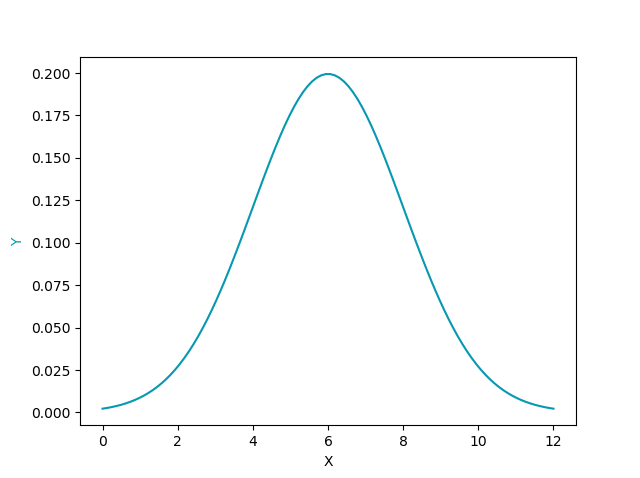
\includegraphics[width=0.6\textwidth]{Normal_clean}
		\end{center}
		
		\begin{definition}
			\label{def:def2}
			Consider a normal distribution $N(\mu, \sigma)$. The \emph{standard value}, or the \emph{Z-score}, of a given $x$ evaluates how many standard deviations away from the mean the given value is. It is computed by $\dfrac{x-\mu}{\sigma}$.
		\end{definition}
	
		\begin{definition}
			\label{def:prob_dist}
			For a given distribution the \emph{probability distribution function} $F(x)$ calculates the probability that a random variable, following the distribution, is less or equal to $x$
			$$F_{X}(x)=\mathbb{P}(x\leq X).$$
		\end{definition}
	
		\begin{definition}
			\label{def:prob_dens}
			The \emph{Probability density function} of a continuous random variable $x$, a probability density function describes the probability a random variable $x$ to appear in any interval. Formally it is defined by
			\begin{align*}
				&\mathbb{P}(x < X \leq x+\Delta)=F_X(x+\Delta)-F_X(x)\\
				&f_X(x)=\lim_{\Delta \rightarrow 0} \frac{F_X(x+\Delta)-F_X(x)}{\Delta}.		
			\end{align*}
		\end{definition}
	
		\begin{definition}
			\label{def:err}
			\emph{The error function} is encountered in integrating the normal distribution, it takes z-score as a parameter and calculates the integral between a fixed point and the mean of the distribution
			$$\operatorname{erf}(z)=\dfrac{2}{\sqrt{\pi}}\int_{0}^{z}e^{-t^{2}}dt.$$
		\end{definition}
	
	\section{Approach}
		This model describes the spreading of a ransomware virus. It calculates the optimal ransom for a ransomware attack, distributed exclusively via botnets, without the key component of spreading to every computer in the network. This variant of the attack is relatively cheap to initiate, but has low efficiency.	We treat the act of decrypting the data of a given computer as a service and the ransom as the service price, respectively. \par
		Consider the distribution of the willingness to pay (WTP) of a given target group. This is the maximum price someone would pay for their data. By putting ourselves in the place of the malware authors, we try to find what the distribution is by examining samples of people and how they respond to a given price. This tests, however, cost us valuable time since the awareness of people rises constantly. We strive to determine how many and how big tests should we conduct in order to model the distribution with reasonable error and in the same time not lose too much time?\par
		For a given size of the sample group, we calculate the error of a set of sample `customers' from the mathematically described function of the demand curve, derived from the distribution of WTP. Starting off low, we gradually expand the sample group size, estimating the expected error, via the Least Squares Approach, at each step.
	\section{Model}
		Here the inner workings of the model are stated in detail, showing how the results and conclusions were reached. The section is divided into two parts, corresponding to the parameters the model explores.
		\subsection{Sample size and error}
			This section describes the mathematical model, used to optimize the error and draw conclusions about the sample size.\par
			We assume people's data value follows a normal distribution and link it to a random variable $p\sim N(500, 150)$. The probability density function (PDF) of a normal distribution $N(\mu, \sigma)$ is $$\frac{1}{\sigma\sqrt{2\pi}}e^{-\frac{(x-\mu)^{2}}{2\sigma^{2}}}.$$\par\noindent
			In order to calculate the demand function $f(k)$ from the PDF for a given price $k$, we need to calculate
			$$\int_{k}^{\infty}f(x)\operatorname{d} x.$$
			\begin{figure}[H]
				\begin{minipage}{0.48\textwidth}
					\centering
					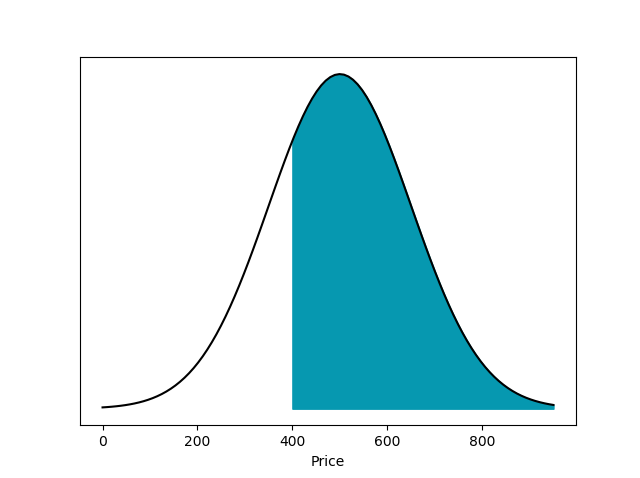
\includegraphics[width=\linewidth]{ND_integral}
					\caption{PDF}\label{Fig:Data1}
				\end{minipage}$\longrightarrow$
				\begin{minipage}{0.48\textwidth}
					\centering
					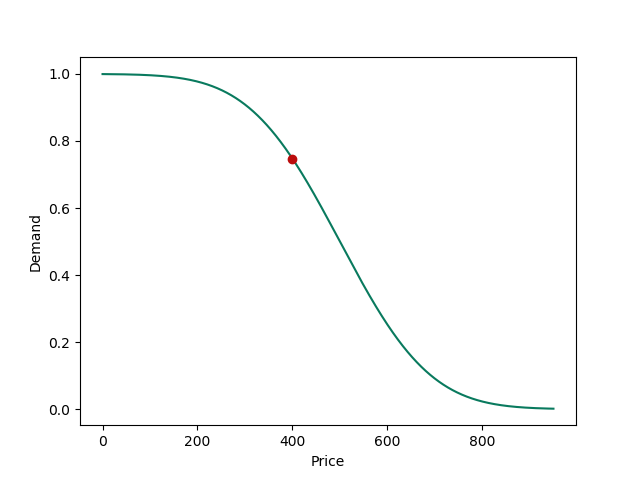
\includegraphics[width=\linewidth]{Sample_point}
					\caption{Price vs Demand}\label{Fig:Data2}
				\end{minipage}
			\end{figure}\par\noindent
			We note that the integral must be calculated up to infinity, but after $k$ reaches $\mu+3\sigma$, the resulting integral is negligibly small. Doing this for the whole probability distribution function gives us the demand curve with respect to what percent of the people would pay. Let us denote the demand curve function with $F(x)$:
			$$
			F(x)=
			\begin{cases}
				\dfrac{1}{2}\left (1-\operatorname{erf}\left (\dfrac{z}{\sqrt{2}}\right )\right ) \text{if } x>\mu,\\
				\\
				\dfrac{1}{2}\left (1+\operatorname{erf}\left (\dfrac{z}{\sqrt{2}}\right )\right ) \text{if } x<\mu.
			\end{cases}
			$$\par
			We aim to optimize the number of people each sample group consists of. Knowing the actual mathematical function we aim to describe gives us the possibility to evaluate the errors from the experimental data with maximum accuracy.
			\begin{figure}[H]
				\begin{minipage}{0.48\textwidth}
					\centering
					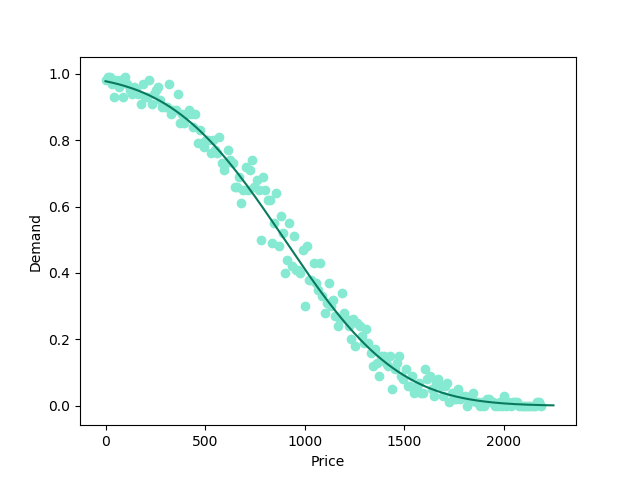
\includegraphics[width=\linewidth]{Exp_and_math_100}
					\caption{Sample size 100}\label{Fig:Data3}
				\end{minipage}\hfill
				\begin{minipage}{0.48\textwidth}
					\centering
					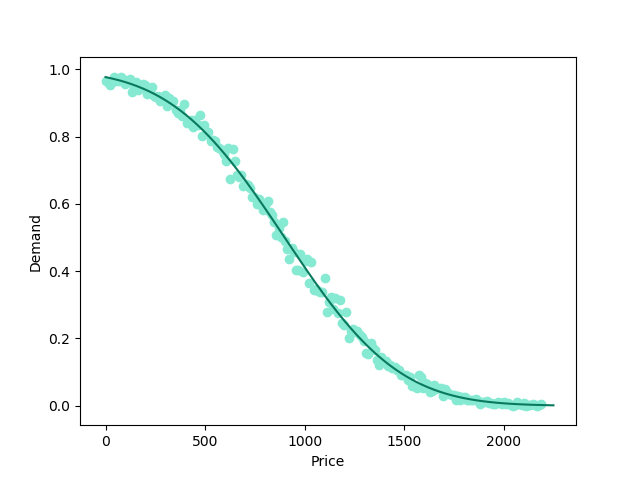
\includegraphics[width=\linewidth]{Exp_and_math_400}
					\caption{Sample size 400}\label{Fig:Data4}
				\end{minipage}
			\end{figure}\par\noindent
			By gathering information on the sample size and the corresponding errors, we plot the changes in the error.
			\begin{figure}[H]
			\begin{minipage}{1.0\textwidth}
				\centering
				\includegraphics[width=0.7\textwidth]{"Error vs sample size 4"}
				\caption{Sample size vs Error}\label{Fig:Data5}
			\end{minipage}
			\end{figure}
		\subsection{Backup function}
			In this section a function, describing the use of backups, is described. The effect on revenue is calculated.\par
			First let us define the backup iterator $b$: 
			$$
			b=
			\begin{cases}
				1 \text{ if the victim has backup},\\
				0 \text{ if the victim does not have backup}
			\end{cases}
			$$
			Now let us define the willingness to pay (WTP) function:
			$$
			P(x)=
			\begin{cases}
			d_{x} \text{ if } b_{i}=0,\\
			c \text{ if } b_{i}=1
			\end{cases}
			$$
			Here the cost of backup is denoted with $c$ and the value of the victim's data - with $d_{x}$.\par
			As earlier, we can calculate the expected probability of people paying a ransom of price $x$
			We assume that the probability that a single victim has backup follows is $p$ and explore how changing this value affects the expected profit. With the gathered data, we create a plot to show the correlation between the two variables
			\begin{center}
				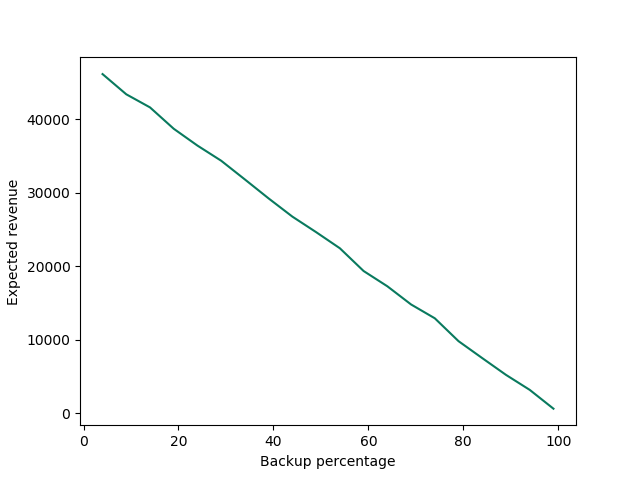
\includegraphics[width=0.55\textwidth]{Revenue_vs_backup}
			\end{center}
			
\section{Results}
	We have explored how the sample size affects the expected error between the statistical and experimental data and have explored how backups affect expected revenue. The model mainly focuses on optimizing the ransom prize, but the author truly believes that in order for us to be able to take countermeasures against ransomware attacks, we need to understand their every move. Putting ourselves in their shoes is essential to the purpose. Additional results, such as the distribution of expected revenue with respect to backup percentages, can help us to draw conclusions how to counteract.
\section{Further development}
	The author considers several future development directions for the project, namely:
	\begin{itemize}
		\item considering the use of backups and its influence on the WTP distribution
		\item expanding the model to describe more complex way of distributing the ransomware
		\item using the results and databases of related studies in order to back the project with real data\cite{paquet2019ransomware}
		\item considering a dynamic pricing model
	\end{itemize}
\section{Acknowledgments}
I want to thank my mentor, Yavor Papazov, and Konstantin Delchev for the enormous help with the choice of the research subject and for providing me with all the necessary material to get familiar with the topic, as well as listening to my questions along the whole way. I extend my gratitude towards Victor Velev, Victor Kolev and Stefan Hadzhistoikov for the support I got from them when I needed it the most. I also want to thank Stanislav Harizanov for the professional expertise.
\nocite{*}
\bibliographystyle{unsrt}
\bibliography{Bibliography}
\end{document}